\section{Problem 4}

\subsection{Question}
Re-run question 2, but this time with proper TFIDF calculations instead of the hack discussed on slide 7 (p. 32).  Use the same 500 words, but this time replace their frequency count with TFIDF scores as computed in assignment \#3. Document the code, techniques, methods, etc. used to generate these TFIDF values.  Upload the new data file to github.\\
\\
Compare and contrast the resulting dendrogram with the dendrogram from question \#2.\\
\\
Note: ideally you would not reuse the same 500 terms and instead come up with TFIDF scores for all the terms and then choose the top 500 from that list, but I'm trying to limit the amount of work necessary.

\subsection{Answer}

With the code in Listing \ref{listing:scaledownmain}, multidimensional scaling (MDS) was used to create a two-dimensional visualization of the blog distance graph. This code calls the {\tt scaledown} function, which is shown in Listing \ref{listing:scaledownfunc}. The algorithm continues until the error factor stops decreasing, as shown in the output in Listing \ref{scaledown}. 

\lstinputlisting[language=Python, caption={main for scaledown}, label=listing:scaledownmain,linerange={306-307},
firstnumber=306]{clusters.py}

\lstinputlisting[language=Python, caption={scaledown function}, label=listing:scaledownfunc,linerange={224-272},firstnumber=224]{clusters.py}

The {\tt scaledown} function returns the coordinates for each of the blogs in 2D space. This data was then used with the {\tt draw2d} function in Listing \ref{listing:draw2d}, which produced the two-dimensional visualation created from the MDS algorithm, as shown in Figure \ref{fig:blogs2d}.

\lstinputlisting[language=Python, caption={draw2d function}, label=listing:draw2d,linerange={274-281},firstnumber=274]{clusters.py}

\begin{figure}[h!]
\centering
\fbox{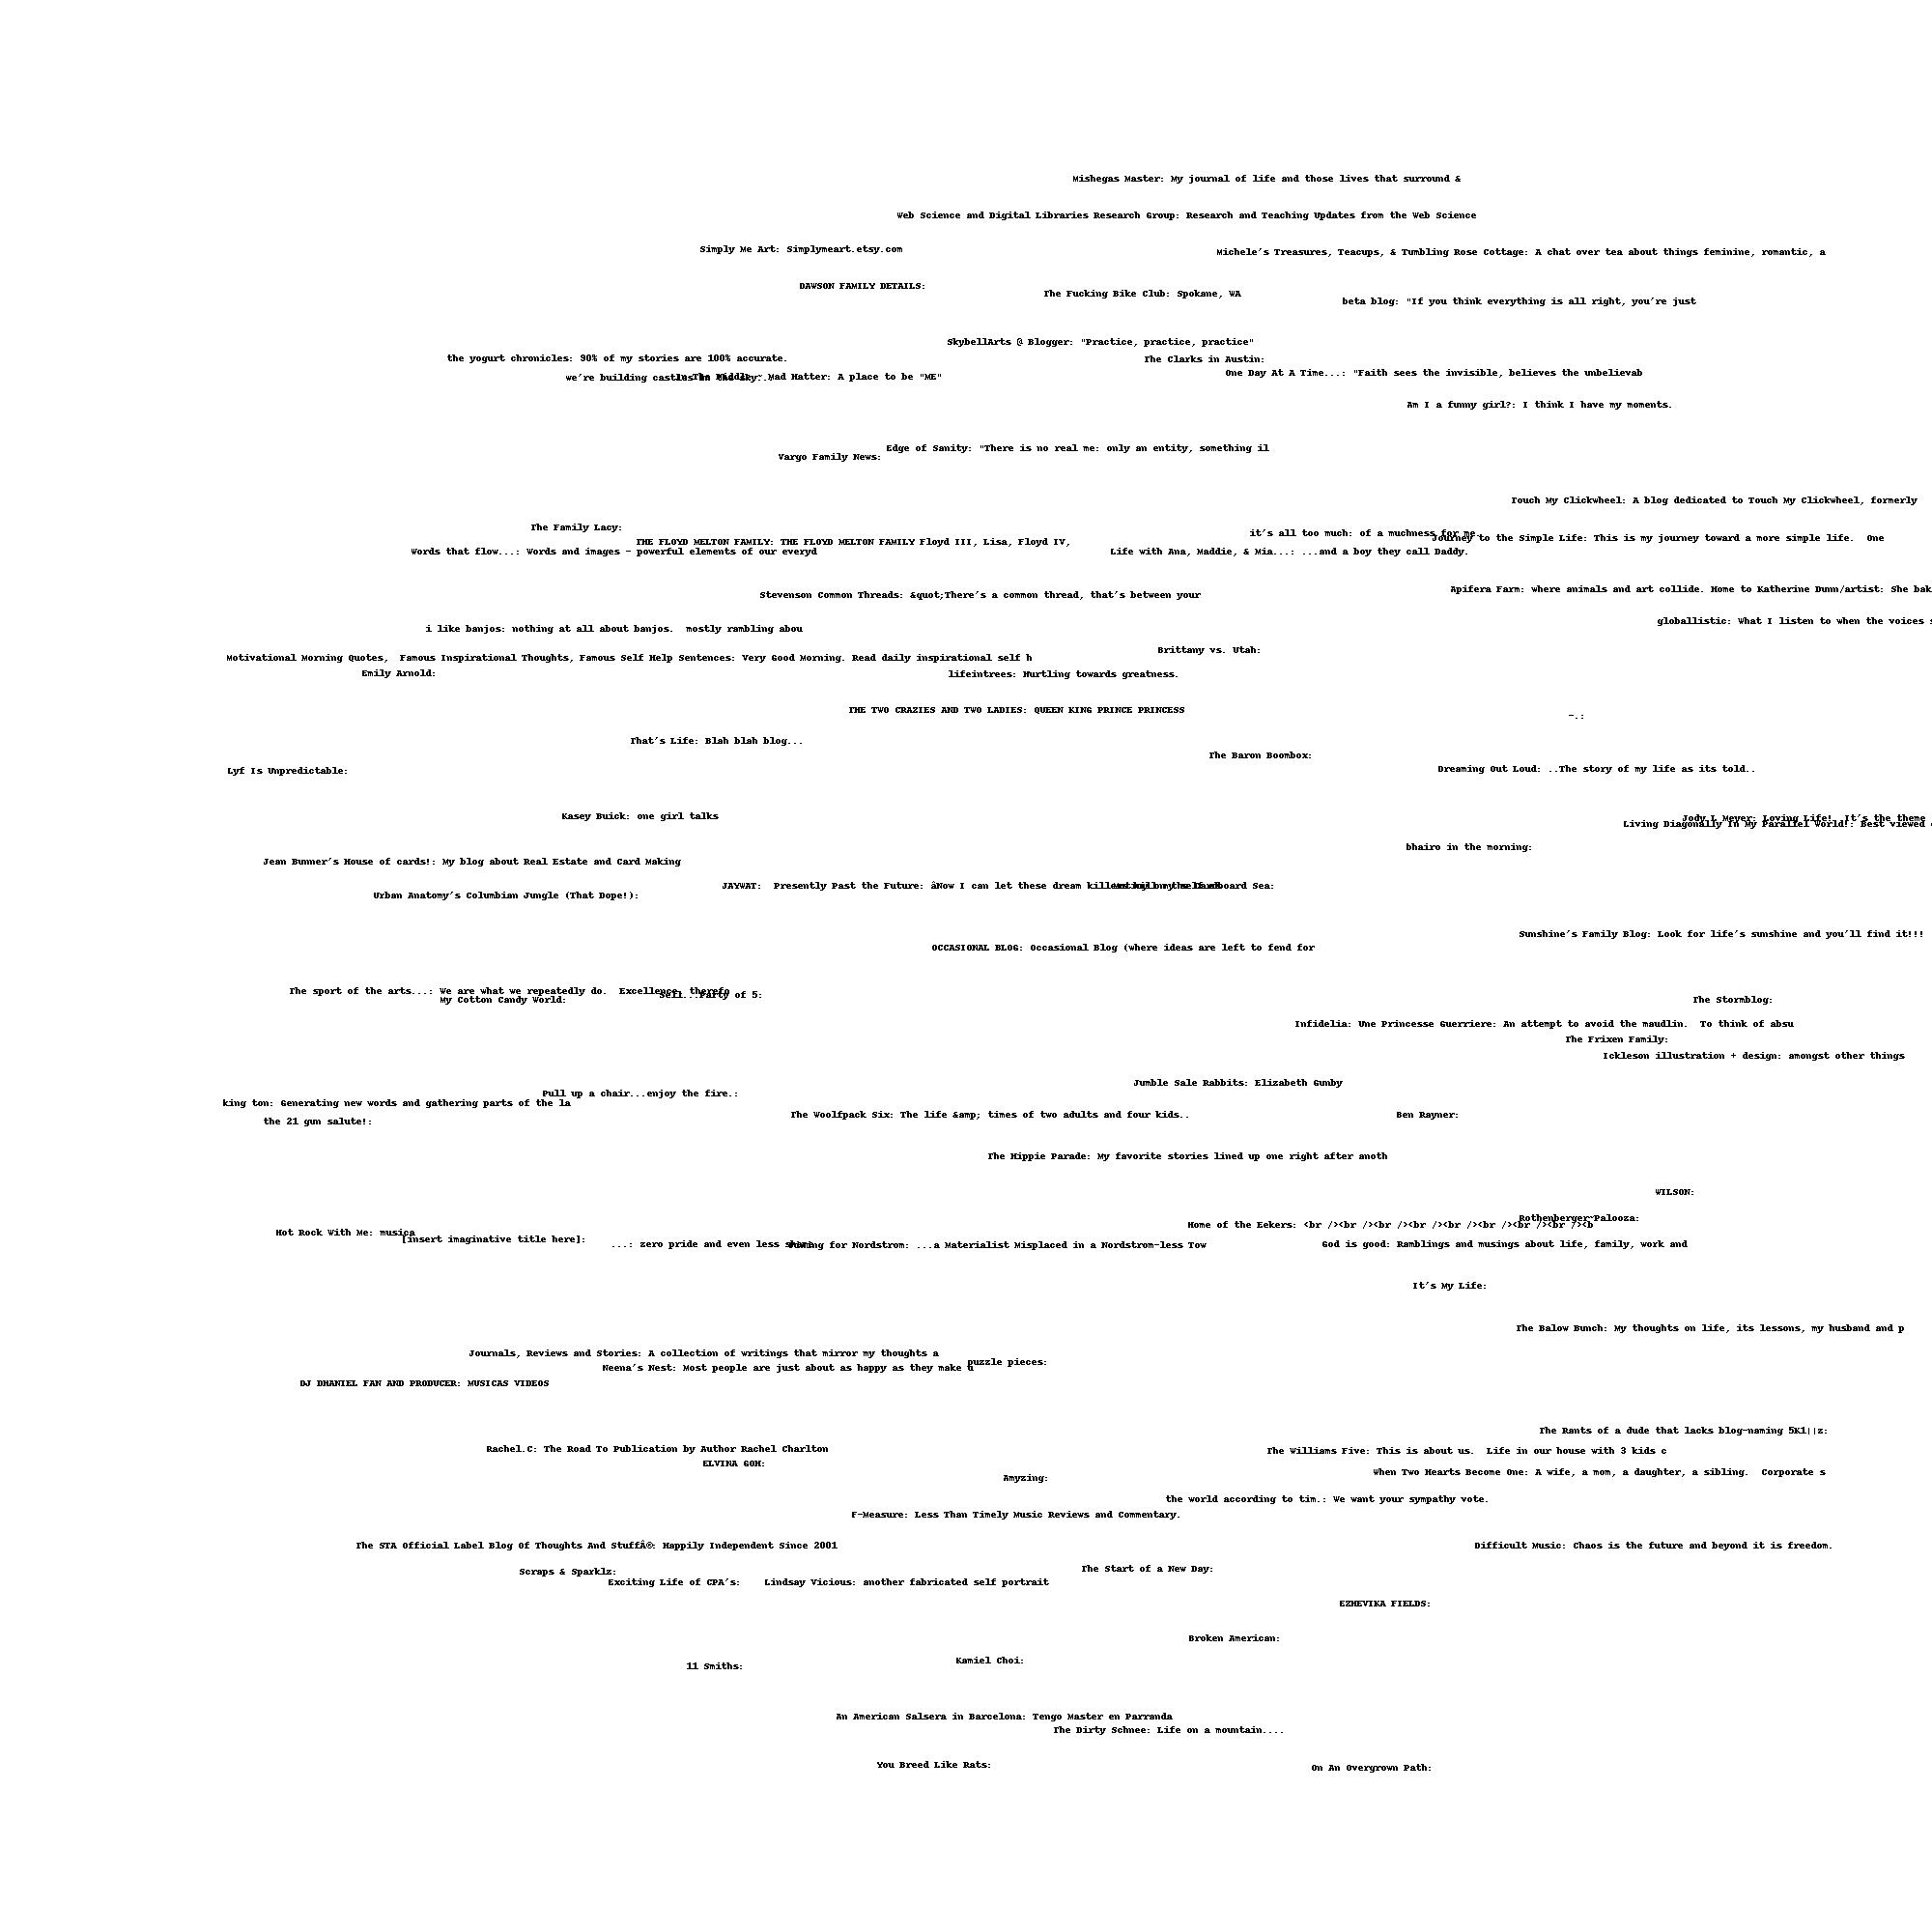
\includegraphics[trim=0 0 0 500, clip, scale=0.2]{q4/blogs2d.jpg}}
\caption{MDS 2d visualization}
\label{fig:blogs2d}
\end{figure}
\clearpage
\lstinputlisting[language=Bash, caption={scaledown output}, label=scaledown]{q4/scaledown.txt}